% Created 2024-07-13 Sat 17:54
% Intended LaTeX compiler: pdflatex
\documentclass[10pt,table,dvipsnames,compress]{beamer}
\usepackage[utf8]{inputenc}
\usepackage[T1]{fontenc}
\usepackage{graphicx}
\usepackage{longtable}
\usepackage{wrapfig}
\usepackage{rotating}
\usepackage[normalem]{ulem}
\usepackage{amsmath}
\usepackage{amssymb}
\usepackage{capt-of}
\usepackage{hyperref}
\usetheme{default}
\useinnertheme{rounded}
\useoutertheme[subsection=false]{miniframes}
\date{}
\title{Jurisdictional risk maps for allocating deforestation}
\title[riskmaps]{Jurisdictional risk maps for allocating deforestation}
\definecolor{darkgreen}{RGB}{34,139,34} % vert moyen
\usepackage{float}
\usepackage{lmodern}
\usepackage{pgf}
\usepackage{color}
\usepackage[english,french]{babel}
\definecolor{vertmoyen}{RGB}{51,110,23} % vert moyen
\definecolor{blueFRB}{HTML}{31859c}
\usecolortheme[named=blueFRB]{structure}
\usepackage{tabularx} % varier la largeur du tableau
\usepackage{layout}
\setlength{\LTleft}{-5cm plus 1 fill}
\setlength{\LTright}{-5cm plus 1 fill}
\usepackage{booktabs}
\usepackage{arydshln} %% dashlines for tabular
\newcommand{\logit}{\text{logit}}
\newcommand{\bs}[1]{\boldsymbol{#1}}
\newcommand{\R}{\textnormal{\sffamily\bfseries R}}
\newcommand{\pkg}[1]{{\fontseries{b}\selectfont #1}}
\newcolumntype{C}[1]{>{\centering\arraybackslash}m{#1}}

\setbeamertemplate{footline}[frame number]
\setbeamertemplate{frametitle}{%
\usebeamerfont{frametitle}\insertframetitle%
\vphantom{g} % To avoid fluctuations per frame
\par
\centering 
\includegraphics[width=\textwidth]{figs/Barre_couleur}
}
\beamertemplatenavigationsymbolsempty

% Logo
\newif\ifplacelogo % create a new conditional
\logo{\ifplacelogo
\includegraphics[width=0.5\textwidth]{figs/partners_logos}\fi}

%Call table of contents at the beginning of each section
\AtBeginSection[]{
\placelogotrue
\begin{frame}
\frametitle{Outline}
\begin{columns}[c]
\begin{column}{0.5\textwidth}
\tableofcontents[sections=1,currentsection]
\vspace{0.5cm}
\tableofcontents[sections=2,currentsection]
\end{column}
\begin{column}{0.5\textwidth}
\tableofcontents[sections=3,currentsection]
\vspace{0.5cm}
\tableofcontents[sections=4,currentsection]
\end{column}
\end{columns}
\end{frame}
\placelogofalse
}

%Call table of contents at the beginning of each subsection
\AtBeginSubsection[]{
\placelogotrue
\begin{frame}
\frametitle{Outline}
\begin{columns}[c]
\begin{column}{0.5\textwidth}
\tableofcontents[sections=1,currentsection, currentsubsection]
\vspace{0.5cm}
\tableofcontents[sections=2,currentsection, currentsubsection]
\end{column}
\begin{column}{0.5\textwidth}
\tableofcontents[sections=3,currentsection, currentsubsection]
\vspace{0.5cm}
\tableofcontents[sections=4,currentsection, currentsubsection]
\end{column}
\end{columns}
\end{frame}
\placelogofalse
}

\hypersetup{
colorlinks=true,
linkcolor=Black,
filecolor=Maroon,
citecolor=Blue,
urlcolor=Maroon}

% Disable monospaced font for URLs
\urlstyle{same}

\hypersetup{
 pdfauthor={Ghislain Vieilledent},
 pdftitle={Jurisdictional risk maps for allocating deforestation},
 pdfkeywords={},
 pdfsubject={},
 pdfcreator={Emacs 29.3 (Org mode 9.6.15)}, 
 pdflang={English}}
\begin{document}

% po4a: environment frame []{_}
% po4a: environment column
% po4a: environment columns
% po4a: environment block {_}
% po4a: command -textcolor {}{_}
% po4a: command -textbf {_}
% po4a: command -url {}
% po4a: command -href {}{_}

% {
%   % Use background image
%   \usebackgroundtemplate{%
%     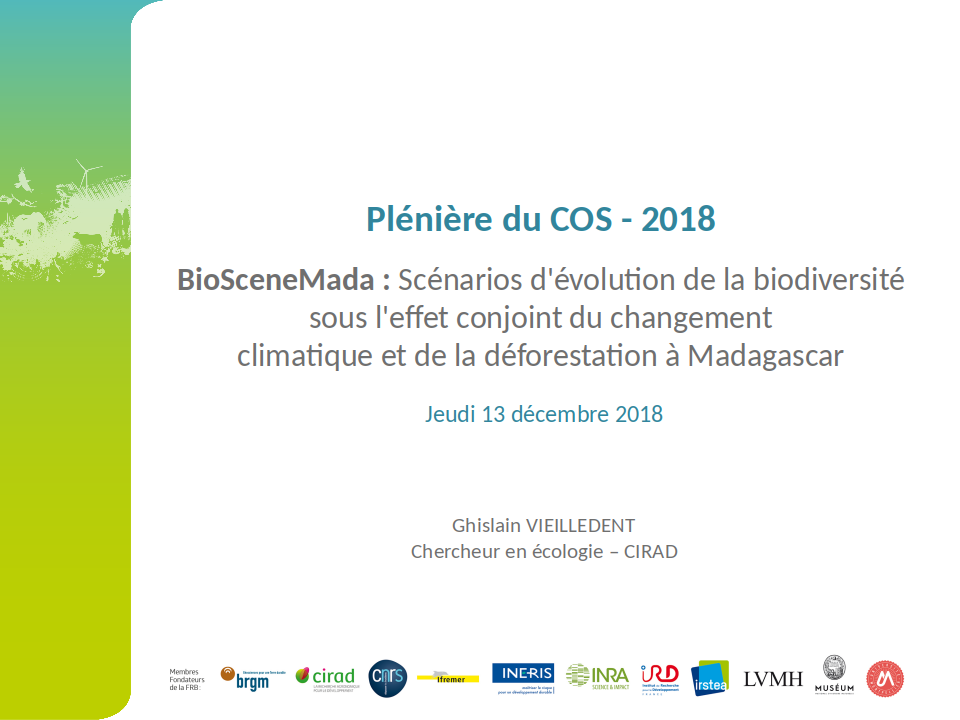
\includegraphics[height=\paperheight,width=\paperwidth]{figs/Masque.png}
%   }
%   \setbeamertemplate{navigation symbols}{}
%   % Remove shadow from block
%   \setbeamertemplate{blocks}[rounded][shadow=false]
%   \begin{frame}[plain]
%   \end{frame}
% }

% Title page
{
  \setbeamertemplate{navigation symbols}{}
  \begin{frame}[plain, noframenumbering]
  \begin{center}
  \small{\textbf{FAO workshop -- Santa Marta (Colombia), July 2024}}
  \end{center}
  \vspace{-0.5cm}
  \titlepage % Presentation first page
  \vspace{-3cm}
  \begin{center}
    
\includegraphics[width=\textwidth]{figs/Barre_couleur}
    
    \vspace{0.25cm}
    
    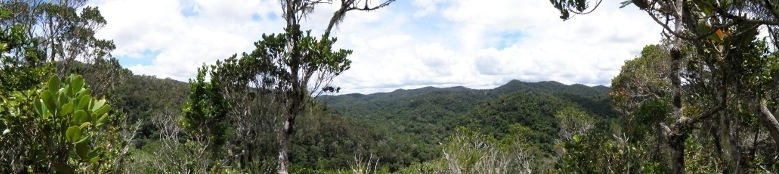
\includegraphics[width=10cm]{figs/Banniere}
    
    \small{Ghislain VIEILLEDENT$^{1}$\hspace{0.25cm}Thomas ARSOUZE$^{1}$\hspace{0.25cm}FAO team$^{2}$}
      
    \vspace{0.25cm}
    
    {\scriptsize
      \begin{tabular}{l}
        $[1]$ \textbf{Cirad} UMR AMAP, $[2]$ \textbf{FAO} Rome and Latin America
      \end{tabular}
    }
    
    
\includegraphics[width=0.8\textwidth]{figs/partners_logos}
    
  \end{center}
  \end{frame}
}

% %%%%%%%%%%%%%%%%%%%%%%%%%%%%%%%%%%%%%%%%%%%%%%%%%%%%%%%%%%%%%%%%

\placelogotrue
\begin{frame}
  \frametitle{Outline}
  \begin{columns}[c]
    \begin{column}{0.5\textwidth}
      \tableofcontents[sections=1]
      \vspace{0.5cm}
      \tableofcontents[sections=2]
    \end{column}
    \begin{column}{0.5\textwidth}
        \tableofcontents[sections=3]
        \vspace{0.5cm}
        \tableofcontents[sections=4]
    \end{column}
  \end{columns}
\end{frame}
\placelogofalse

\section{Introduction}
\label{introduction}
\subsection{Improving certification methodologies}
\label{improving-certification-methodologies}
\begin{frame}[label=several-criticisms-to-project-based-approach]{Several criticisms to project-based approach}
Several criticisms were addressed to previous REDD+ methodologies for carbon credit certification accusing them to oversell credits.

\begin{itemize}
\item \textbf{Non-additionnality}: Emissions reductions would have happened anyway. Inflated project-level baselines. Jurisdictional reference levels are reasonably good predictors of future trends.
\item \textbf{Leakage}: The larger the area covered by a REDD+ initiative, the lower the leakage risk.
\item \textbf{Reversal}: Jurisdictions are less likely than projects to have their forest carbon stocks decimated by a disturbance event.
\end{itemize}

Frances Seymour (WRI): \href{https://www.wri.org/insights/insider-4-reasons-why-jurisdictional-approach-redd-crediting-superior-project-based}{4 Reasons Why a Jurisdictional Approach for REDD+ Crediting Is Superior to a Project-Based Approach}.
\end{frame}

\begin{frame}[label=new-jurisdictional-approach]{New jurisdictional approach}
\begin{block}{Deforestation intensity}
\begin{itemize}
\item Baseline activity data or Forest Reference Emission Level at the jurisdictional level
\item Amount of deforestation.
\item Deforestation ``quantity'' or ``intensity''.
\end{itemize}
\end{block}

\begin{block}{Spatial deforestation risk}
\begin{itemize}
\item Map of the deforestation risk at the jurisdictional level.
\item Spatial relative probability of deforestation.
\item Deforestation ``location''.
\end{itemize}
\end{block}
\end{frame}

\subsection{Allocating deforestation to projects}
\label{allocating-deforestation-to-projects}
\begin{frame}[label=risk-map-at-the-jurisdictional-level]{Risk map at the jurisdictional level}
\begin{columns}
\begin{column}{0.5\columnwidth}
\begin{block}{Objectives}
\begin{itemize}
\item Identifying hot-spots/cold-spots of deforestation.
\item Classifying forest pixels by risk of being deforested.
\item One unique model for the whole jurisdiction (no methodological discrepancies between projects).
\item Use this map to allocate deforestation (estimated for the jurisdiction) per project.
\end{itemize}
\end{block}
\end{column}

\begin{column}{0.5\columnwidth}
\begin{figure}[htbp]
\centering
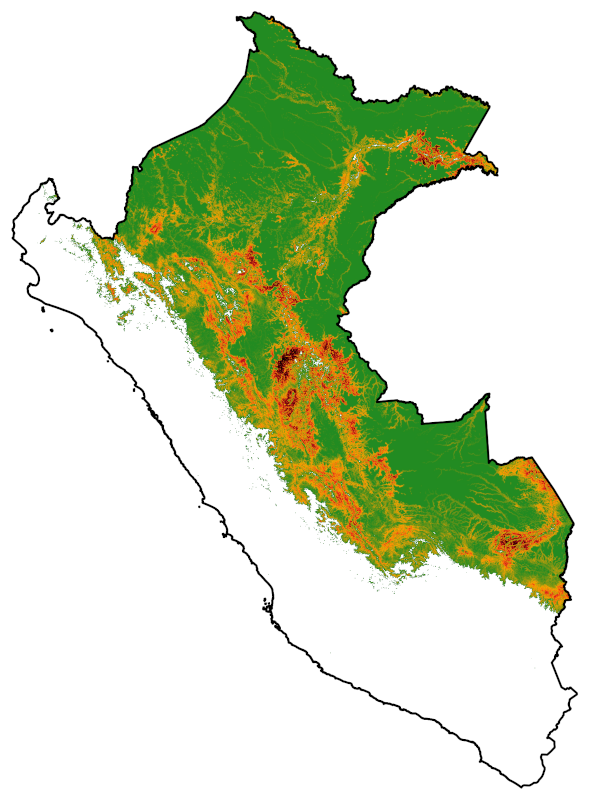
\includegraphics[width=4cm]{figs/prob_PER.png}
\caption{Map of the deforestation risk for Perou.\newline \textcolor{darkgreen}{Green}: low, \textcolor{red}{Red}/\textbf{Black}: high.}
\end{figure}
\end{column}
\end{columns}
\end{frame}

\begin{frame}[label=allocating-deforestation-to-projects]{Allocating deforestation to projects}
\begin{itemize}
\item Jurisdictional risk map: a map with class of deforestation risk.
\item Obtaining a deforestation density map:\newline Class of defor. risk [1, 2, \ldots{}, \(I\)] \(\rightarrow\) Defor. density (ha/yr/pixel).
\item Can be used to allocate deforestation per project.
\end{itemize}

\begin{figure}[htbp]
\centering
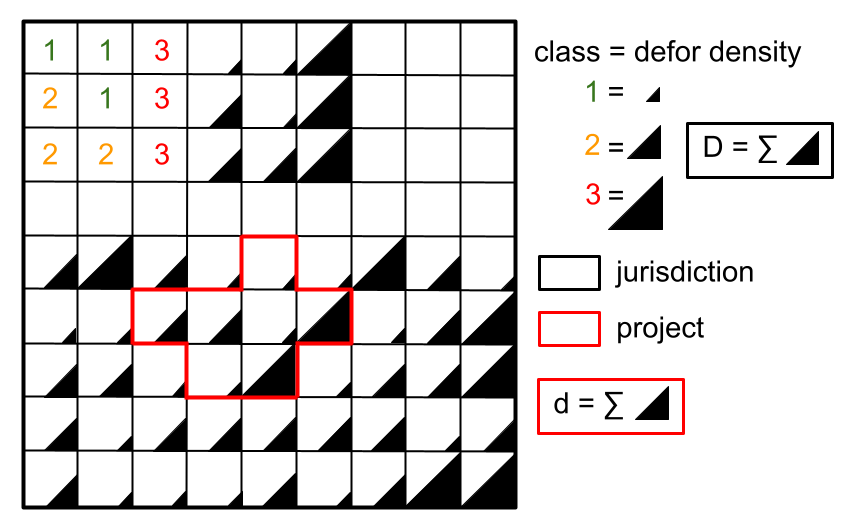
\includegraphics[width=8cm]{figs/get_started/allocation.png}
\caption{Allocating deforestation to projects within the jurisdiction.}
\end{figure}
\end{frame}

\section{Verra methodology for risk mapping}
\label{verra-methodology-for-risk-mapping}
\subsection{VT0007 tool}
\label{vt0007-tool-1}
\begin{frame}[label=vt0007-tool-2]{VT0007 tool}
\begin{itemize}
\item Developed by Clark University (J. R. Eastman and R. G. Pontius Jr.) for Verra.
\item \textbf{Aim}: Obtaining the best risk map possible at the jurisdictional level.
\end{itemize}

\begin{block}{Basic steps}
\begin{enumerate}
\item Use a reasonably good reference model to map the deforestation risk.
\item Let the user propose alternative maps from alternative models.
\item Validation step: check that alternative models are better than the benchmark model.
\item Use the best alternative map to allocate deforestation.
\end{enumerate}
\end{block}
\end{frame}

\begin{frame}[label=modelling-periods]{Modelling periods}
\begin{center}
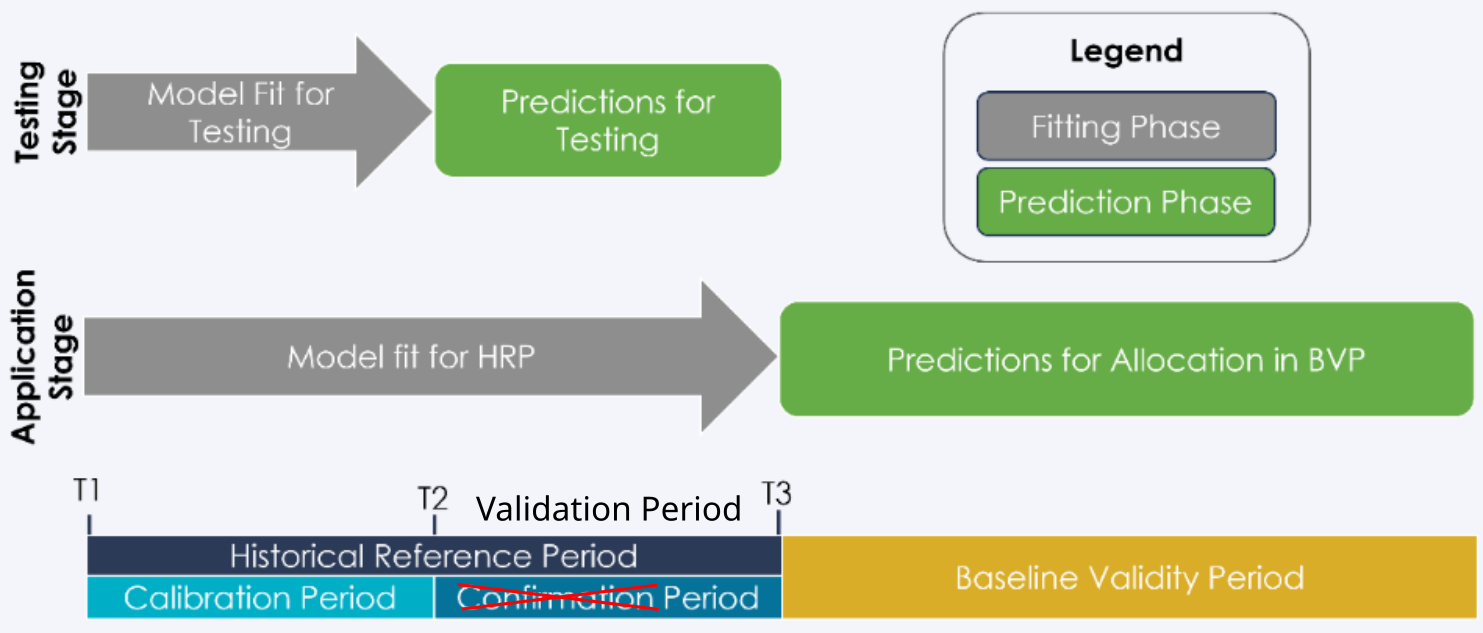
\includegraphics[width=9cm]{figs/get_started/periods.png}
\end{center}

\begin{itemize}
\item Three dates: t1, t2, t3.
\item Four periods: calibration, validation, historical, (baseline validity period).
\item Why different periods: model predictions must be compared with \textbf{independent data} (validation period).
\item To forecast after t3, we want to use as much data as possible (historical period).
\end{itemize}
\end{frame}

\subsection{Benchmark model}
\label{benchmark-model-1}
\begin{frame}[label=benchmark-model-2]{Benchmark model}
\begin{itemize}
\item Benchmark model or reference model.
\item A reasonably good deforestation model (better than a null model).
\item Assuming a \emph{decrease of deforestation with distance to forest edge} (commonly admitted).
\item And a \emph{different model between subjurisdictions} (regional variability).
\end{itemize}

\begin{figure}[htbp]
\centering
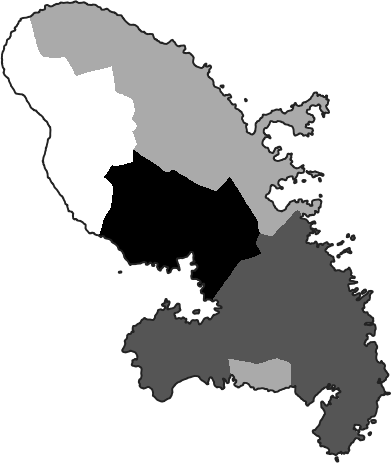
\includegraphics[width=3.5cm]{figs/subj.png}
\caption{Subjurisdictions in Martinique (MTQ)}
\end{figure}
\end{frame}

\begin{frame}[label=distance-threshold]{Distance threshold}
\begin{itemize}
\item Identify the distance to forest edge below which \textbf{99.5\%} of the deforestation occur.
\item Use this distance to define the first class of risk (class 1).
\end{itemize}

\begin{center}
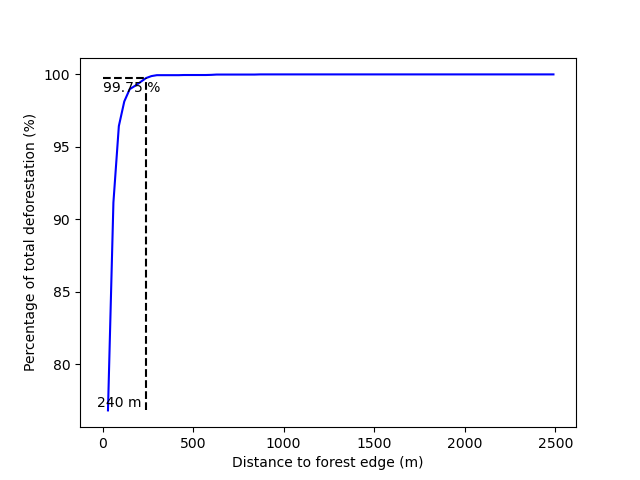
\includegraphics[width=8cm]{figs/get_started/perc_dist.png}
\end{center}
\end{frame}

\begin{frame}[label=from-distance-to-risk-class]{From distance to risk class}
\begin{itemize}
\item Distances below the threshold are transformed into classes of deforestation risk.
\item A geometric series is used for that, ensuring that classes have a wider range for bigger distances.
\item We define 29 additional classes of risk from 2 to 30 (class 1 has already been defined).
\end{itemize}

\begin{center}
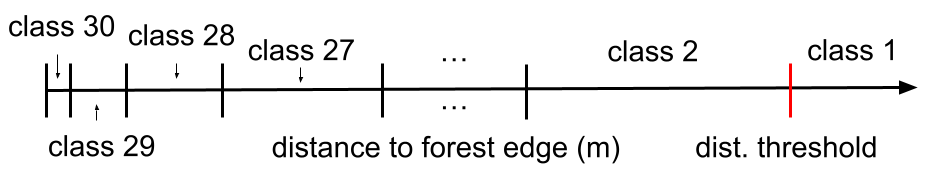
\includegraphics[width=10cm]{figs/dist_class.png}
\end{center}
\end{frame}

\begin{frame}[label=classes-from-subjurisdictions-1]{Classes from subjurisdictions}
\begin{itemize}
\item Each subjurisdiction get a number from 1 to (potentially) 999.
\item We combine classes derived from distance with subjurisdictions in the following way: \(\textbf{DD}\text{SSS}\), with \textbf{DD} the distance class and SSS the subjurisdiction number.
\item We obtain classes going from 01001 to potentially 30999 if there are 999 subjurisdictions.
\item So for 10 subjurisdictions, we obtain \textasciitilde{}300 classes (but some distance classes might be missing).
\end{itemize}
\end{frame}

\begin{frame}[label=classes-from-subjurisdictions-2]{Classes from subjurisdictions}
\begin{itemize}
\item Following these steps, we obtain a map at the jurisdictional level where each forest pixel belongs to a given class of deforestation risk.
\item Area in dark green: classes \(\mathbf{1}\text{SSS}\), beyond the deforestation threshold.
\end{itemize}

\begin{center}
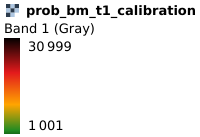
\includegraphics[width=3cm]{figs/prob_bm_t1_legend.png}  
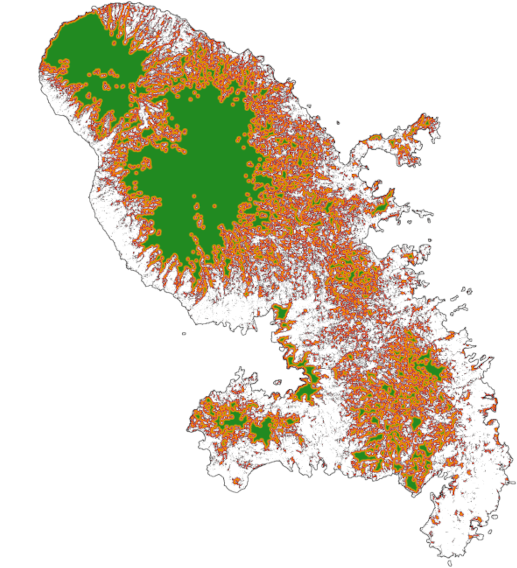
\includegraphics[width=5cm]{figs/prob_bm_t1.png}
\end{center}
\end{frame}

\begin{frame}[label=deforestation-density-1]{Deforestation density}
\begin{itemize}
\item Each class \(i\) has an associated \textbf{deforestation probability}: \(\theta_{m,i} = d_{i} / n_{i}\) (unitless), with \(d_{i}\) the number of deforested pixels during the period, and \(n_{i}\) the number of forest pixels at the beginning of the period.
\item \textbf{Quantity adjustment \(\rho\)}: \(\theta_{a,i} = \rho \theta_{m,i}\), so that total predicted deforestation = observed (or expected) deforestation. For the benchmark model for the calibration and historical periods, \(\rho=1\).
\item \textbf{Deforestation density (in ha/yr per pixel)} computed as \(\delta_{i} = \theta_{a,i} \times A / T\). \(A\): pixel area (in ha), \(T\): time-interval of the period (in yr).
\item The deforestation density is used to predict the amount of deforestation for each pixel belonging to a given class of deforestation risk.
\end{itemize}
\end{frame}

\begin{frame}[label=deforestation-density-2]{Deforestation density}
\begin{table}[htbp]
\caption{\label{tab-defrate}Deforestation rates for each class of deforestation risk (numbers truncated to three decimal digits).}
\small
\begin{tabular}{rrrrrrrr}
\toprule
cat & \(n_i\) & \(d_i\) & \(\theta_{m,i}\) & \(\theta_{a,i}\) & \(T\) & \(A\) & \(\delta_{i}\)\\[0pt]
\midrule
1001 & 33433 & 0 & 0.0 & 0.0 & 10 & 0.09 & 0.0\\[0pt]
1002 & 12965 & 0 & 0.0 & 0.0 & 10 & 0.09 & 0.0\\[0pt]
1003 & 91686 & 19 & 2.072e-04 & 2.072e-04 & 10 & 0.09 & 1.865e-06\\[0pt]
1004 & 82279 & 5 & 6.076e-05 & 6.076e-05 & 10 & 0.09 & 5.469e-07\\[0pt]
2001 & 1373 & 0 & 0.0 & 0.0 & 10 & 0.09 & 0.0\\[0pt]
\bottomrule
\end{tabular}
\end{table}

\textbf{Deforestation density (in ha/yr per pixel)} computed as \(\delta_{i} = \theta_{a,i} \times A / T\)
\end{frame}

\begin{frame}[label=deforestation-density-3]{Deforestation density}
Deforestation density can be used to allocate deforestation to projects within a jurisdiction.

\begin{figure}[htbp]
\centering
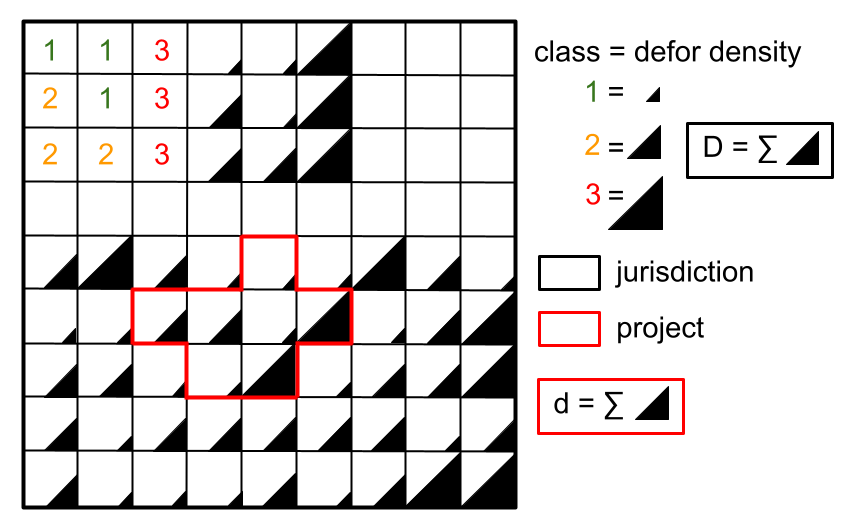
\includegraphics[width=8cm]{figs/get_started/allocation.png}
\caption{Allocating deforestation to projects within the jurisdiction.}
\end{figure}
\end{frame}

\subsection{Alternative models and validation}
\label{alternative-models-and-validation}
\begin{frame}[label=alternative-models-1]{Alternative models}
\begin{itemize}
\item Alternative maps from alternative models must be compared with the benchmark model.
\item The alternative model can be of different forms: geoprocessing model (moving window), statistical model (iCAR, GLM, RF).
\item E.g. Clark Labs propose the MLP (Multi-Layer Perceptron) statistical model in the Land Change Modeller module of the \href{https://clarklabs.org/terrset/}{TerrSet} software.
\end{itemize}
\end{frame}

\begin{frame}[label=alternative-models-2]{Alternative models}
\begin{itemize}
\item A risk map with deforestation densities derived from the alternative model must be provided.
\end{itemize}

\begin{figure}[htbp]
\centering
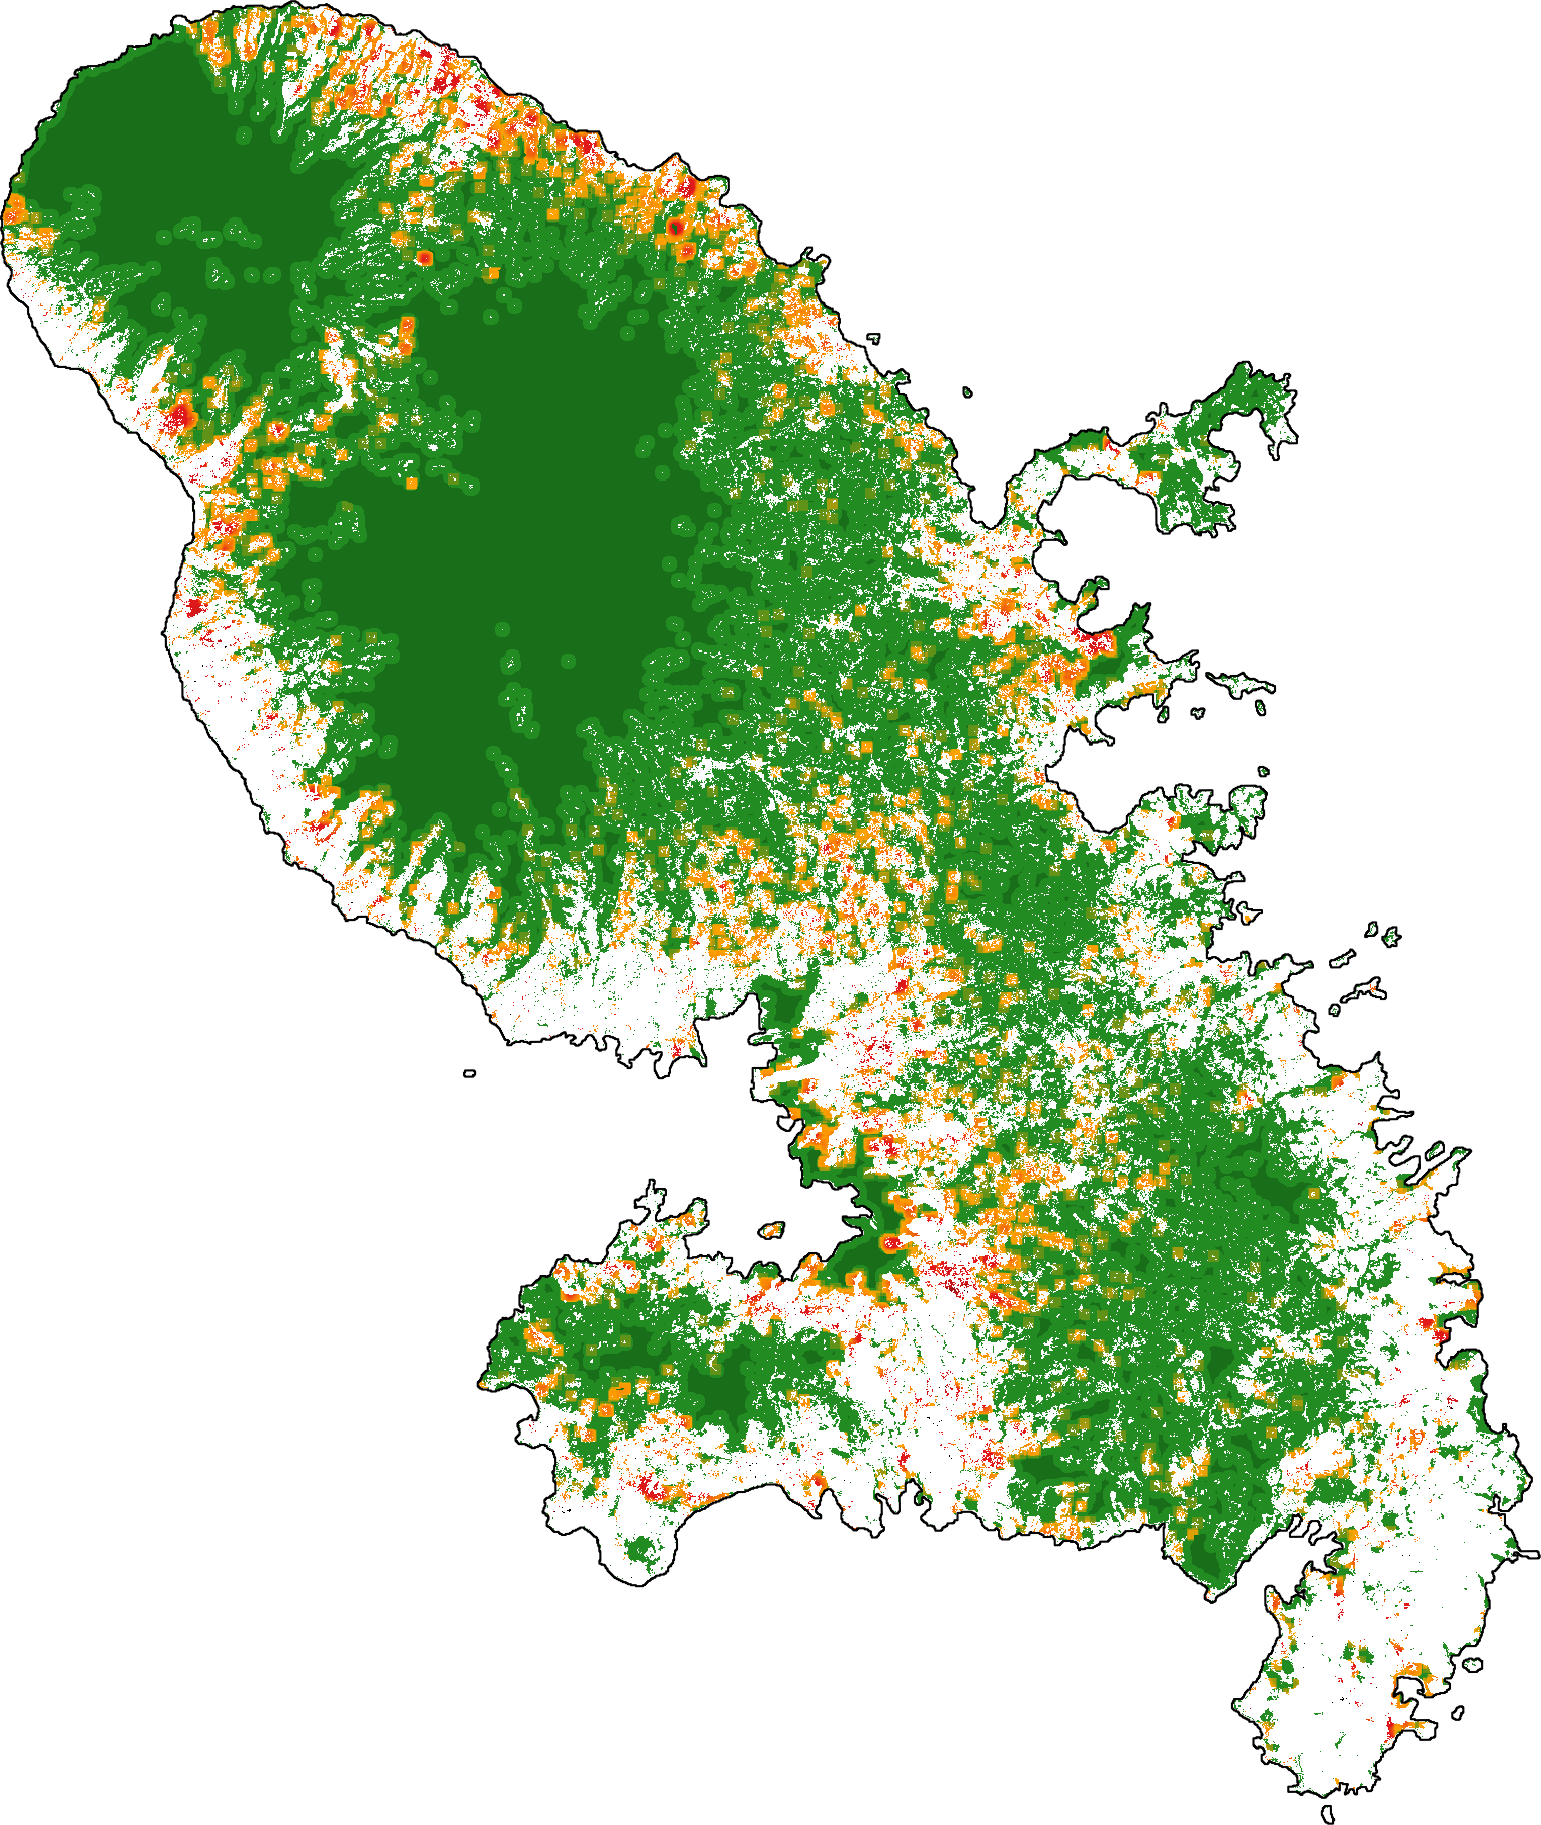
\includegraphics[width=4.5cm]{figs/prob_mw_11_t1.png}
\caption{Risk map obtained with a moving window model.}
\end{figure}
\end{frame}

\begin{frame}[label=validation-procedure-1]{Validation procedure}
\begin{itemize}
\item Comparing predicted vs. observed deforestation (in ha) in a coarse grid.
\item For a given period of time.
\end{itemize}

\begin{figure}[htbp]
\centering
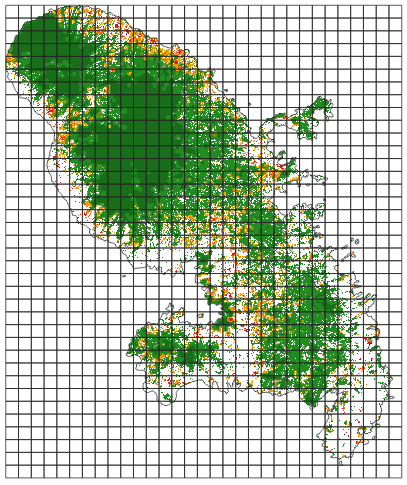
\includegraphics[width=4.5cm]{figs/grid.png}
\caption{Coarse grid covering the area of interest.}
\end{figure}
\end{frame}

\begin{frame}[label=validation-procedure-2]{Validation procedure}
\begin{itemize}
\item Comparing predicted vs. observed deforestation.
\item Performance indices: \(R^2\), and median of absolute error (MedAE).
\end{itemize}

\begin{center}
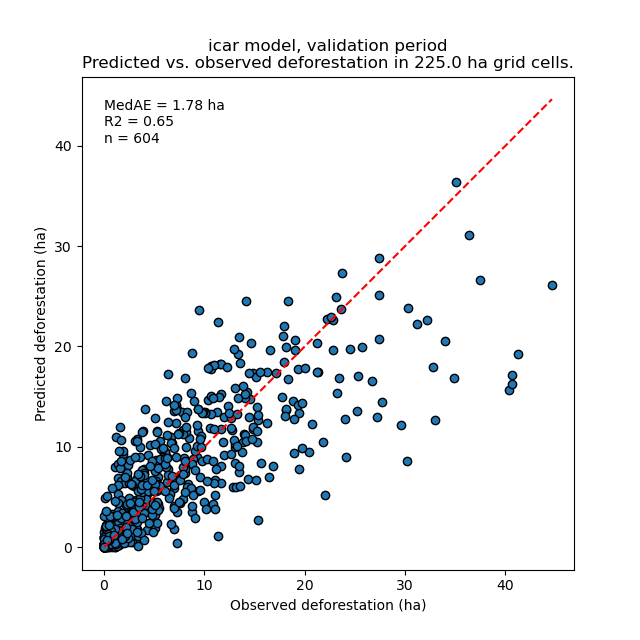
\includegraphics[width=6.5cm]{figs/get_started/pred_obs_icar_validation_50.png}
\end{center}
\end{frame}

\begin{frame}[label=validation-procedure-3]{Validation procedure}
\begin{itemize}
\item Performance indices are computed for each model.
\item The model with the higher \(R^2\) and the lower MedAE is selected.
\end{itemize}

\begin{table}[htbp]
\caption{\label{tab-indices}Performance indices.}
\small
\begin{tabular}{rllrrrr}
\toprule
ncell & period & model & MedAE & R2 & RMSE & wRMSE\\[0pt]
\midrule
604 & validation & bm & 2.71 & 0.43 & 6.08 & 6.22\\[0pt]
604 & validation & icar & 1.78 & 0.65 & 4.79 & 4.59\\[0pt]
604 & validation & glm & 2.39 & 0.38 & 6.39 & 6.52\\[0pt]
604 & validation & rf & 2.09 & 0.50 & 5.69 & 5.74\\[0pt]
604 & validation & mw\_11 & 2.34 & 0.56 & 7.66 & 6.83\\[0pt]
604 & validation & mw\_21 & 2.51 & 0.56 & 7.54 & 6.66\\[0pt]
\bottomrule
\end{tabular}
\end{table}
\end{frame}

\begin{frame}[label=validation-procedure-4]{Validation procedure}
\begin{center}
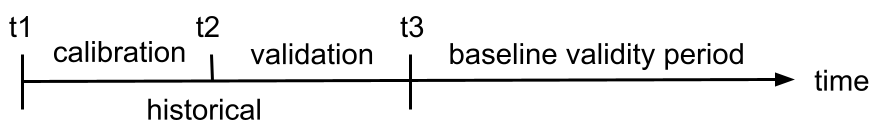
\includegraphics[width=.9\linewidth]{figs/periods.png}
\label{tab-periods}
\end{center}

\begin{itemize}
\item We can compare predicted vs. observed deforestation for three time periods: \textbf{calibration}, \textbf{validation}, and \textbf{historical period}.
\item To estimate model performance at forecasting deforestation in the future: \textbf{predicted vs. observed deforestation} for the \textbf{validation period} with a model fitted over the \textbf{calibration period}.
\item This way, we use \textbf{independent observations} of deforestation for model validation (observed deforestation over the validation period have not be used to calibrate the model).
\item Verra's methodology: the alternative model must be better for both the calibration and validation periods.
\end{itemize}
\end{frame}

\section{Software for deforestation risk mapping}
\label{software-for-deforestation-risk-mapping}
\subsection{Verra/Clark Labs software}
\label{verra-clark-labs-software-1}
\begin{frame}[label=verra-clark-labs-software-2]{Verra/Clark Labs software}
\begin{center}
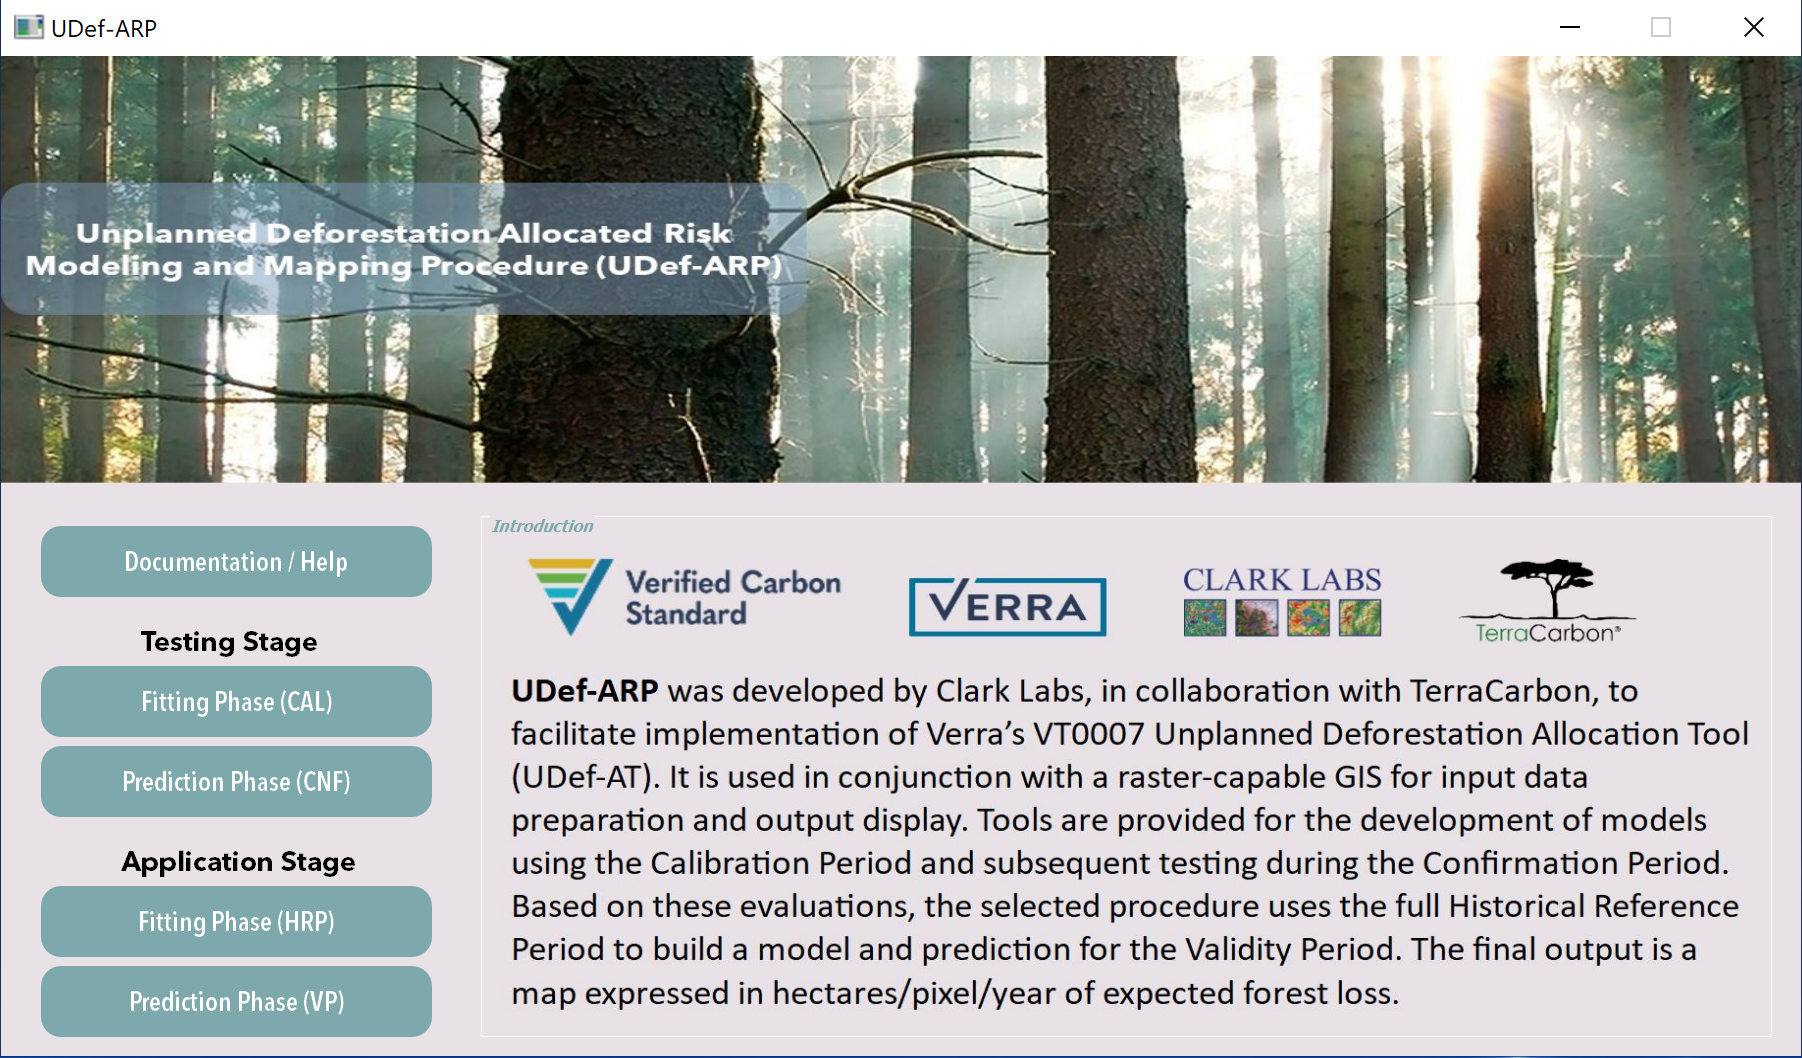
\includegraphics[width=9cm]{figs/verra_tool.png}
\end{center}

\centering Standalone app: \url{https://github.com/ClarkCGA/UDef-ARP} \\[0pt]
\centering QGIS plugin: \url{https://github.com/ClarkCGA/UDef-ARP-Plugin}
\end{frame}

\begin{frame}[label=verra-clark-labs-software-3]{Verra/Clark Labs software}
\begin{center}
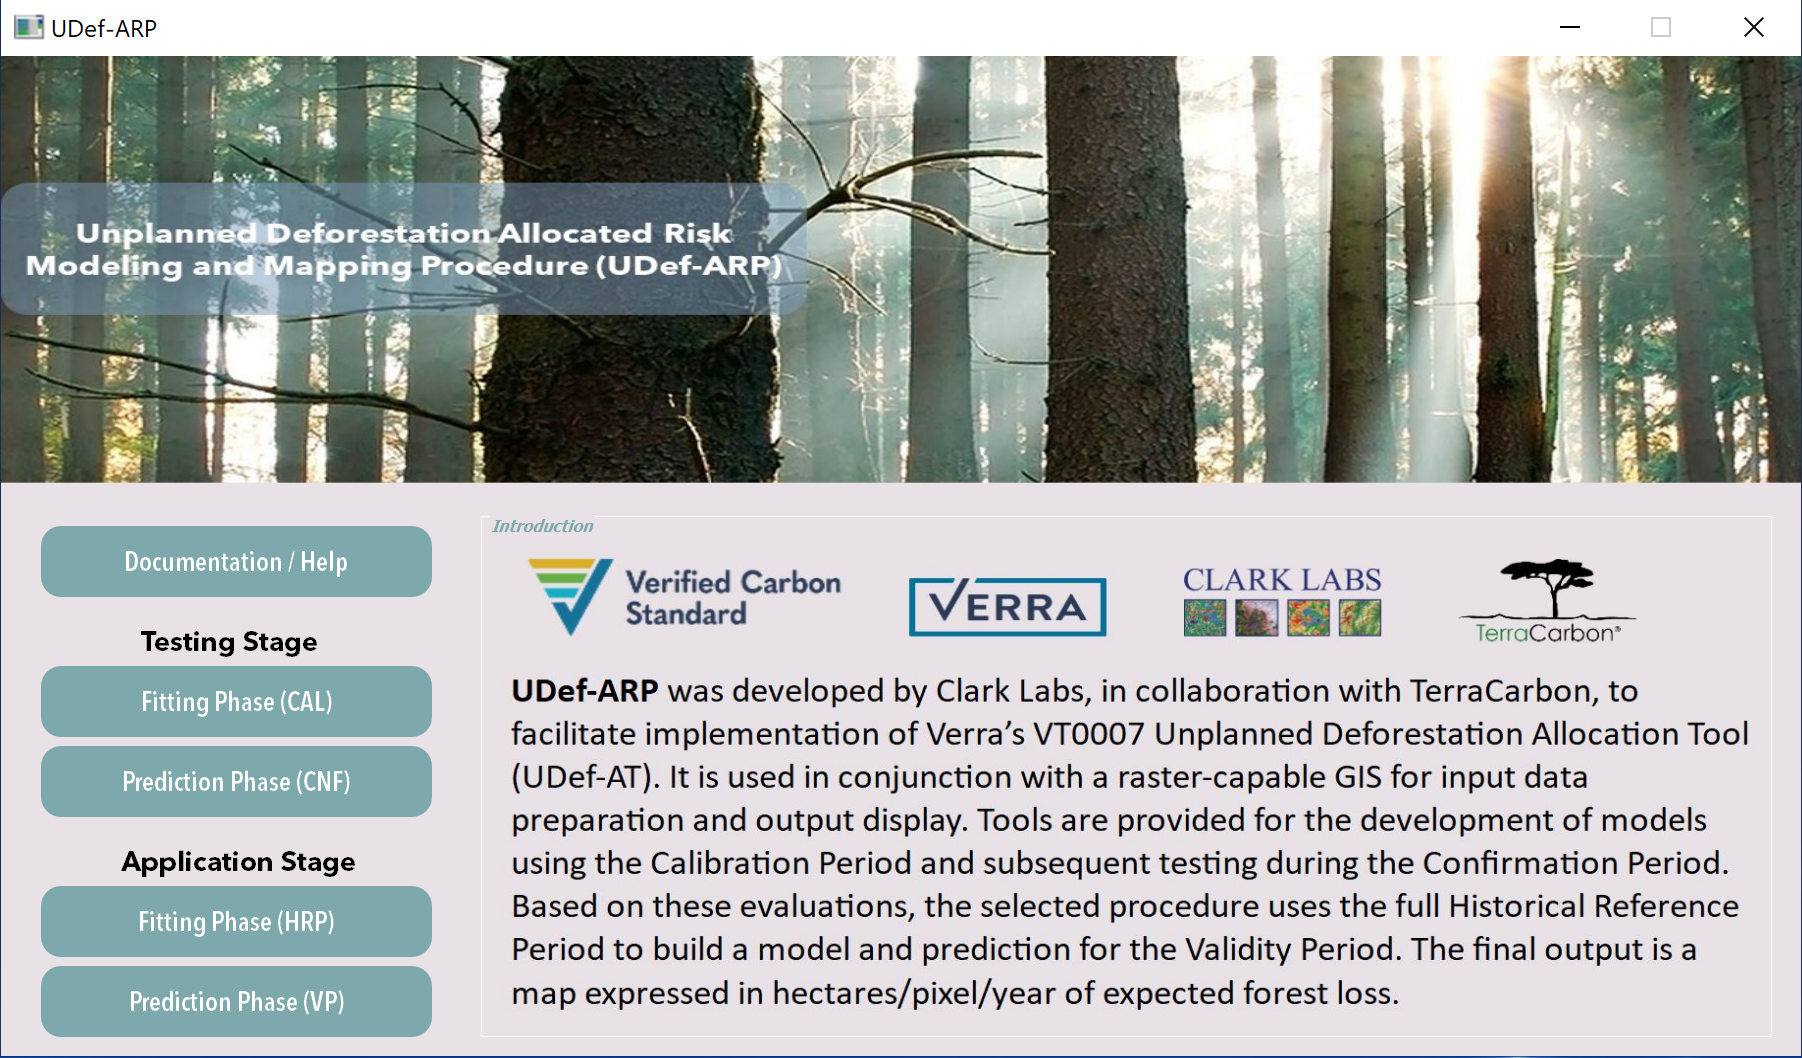
\includegraphics[width=6cm]{figs/verra_tool.png}
\end{center}

\begin{itemize}
\item User must provide rasters: forest cover change, distance to forest edge at several dates, subjurisdictional borders, alternative risk maps at several dates.
\item Using this data, the UDef-ARP provides the basis:
\begin{itemize}
\item for developing a benchmark model.
\item for comparing the benchmark and alternative models.
\end{itemize}
\end{itemize}
\end{frame}

\begin{frame}[label=limitations-1]{Limitations}
\begin{itemize}
\item No tool to help prepare the data.
\item No tool to help develop the \textbf{alternative models}.
\item Windows only (at the moment).
\item Require a computer with high RAM for large jurisdiction: all rasters are stored in RAM during processing. Therefore, large jurisdictions will \textbf{require substantial RAM allocations} (e.g., 64Gb).
\item Use of Float data for risk maps with deforestation density (ha/pixel/yr): \textbf{large space on disk}.
\item Documentation in English only, \textbf{no translations available}.
\item Recent tool, some feedbacks from users (e.g. Fronterra): \href{https://www.linkedin.com/posts/fron-terra\_forest-carbon-climatechange-activity-7179166090042732544-YnAK?utm\_source=share\&utm\_medium=member\_desktop}{Post 1}, \href{https://www.linkedin.com/posts/fron-terra\_forest-carbon-climatechange-activity-7179721587267371008-PRXr?utm\_source=share\&utm\_medium=member\_desktop}{Post 2}, \href{https://www.linkedin.com/posts/fron-terra\_carbon-climatechange-verra-activity-7180971577746862080-rolc?utm\_source=share\&utm\_medium=member\_desktop}{Post 3}.
\end{itemize}
\end{frame}

\subsection{Existing software for alternative models}
\label{existing-software-for-alternative-models-1}
\begin{frame}[label=existing-software-for-alternative-models-2]{Existing software for alternative models}
\begin{itemize}
\item \href{https://csr.ufmg.br/dinamica/}{Dinamica EGO}: Universidade Federal de Minas Gerais, Brazil.
\item \href{https://clarklabs.org/terrset/land-change-modeler/}{Land Change Modeler}: Clark Labs, Clark University, Worcester, USA.
\item \href{https://www.environmentalgeography.nl/site/data-models/data/clue-model/}{CLUE}: Institute for Environmental Studies, Vrije Universiteit, Amsterdam, Netherlands .
\end{itemize}

\vspace{0.25cm}

\textbf{Great programs} with many applications. Many scientific studies, published in a large number of scientific articles, have used these programs.
\end{frame}

\subsection{Limitations}
\label{limitations-2}
\begin{frame}[label=limitations-3]{Limitations}
\begin{itemize}
\item Not all are open source (e.g. Dinamica EGO and LCM): \textbf{transparency}.
\item Not all are free (e.g. LCM): but discount for student and developing countries.
\item Not all allow scripting (e.g. LCM, CLUE): \textbf{reproducibility}.
\item Might not work with high resolution (<= 30 m) rasters on large jurisdictions (country scale).
\item Limited number of statistical models for modelling land use change: limited accuracy and over-fitting.
\end{itemize}

\vspace{0.25cm}

See \textbf{Vieilledent et al.} 2021, \emph{JOSS}, doi: \href{https://doi.org/10.21105/joss.02975}{10.21105/joss.02975} for more details.
\end{frame}

\begin{frame}[label=limitations-4]{Limitations}
\begin{itemize}
\item Verra's methodology includes \textbf{several steps} (calibration, validation, forecast), which must be \textbf{repeated} (model, period).
\item It must be possible to follow Verra's methodology with one of these programs (given some requirements, such as high RAM computer).
\item But it would require a lot of work for the user to adapt the use of the program to Verra's methodology (e.g. validation step with coarse grid).

\item \textbf{Note}: in the documentation for UDef-ARP, Clark Labs indicates plans to offer a utility to facilitate the creation of vulnerability maps for alternative models in the near future.
\end{itemize}
\end{frame}

\section{Conclusion}
\label{conclusion}
\subsection{A not so simple methodology}
\label{a-not-so-simple-methodology-1}
\begin{frame}[label=summary]{Summary}
\begin{itemize}
\item We need a \textbf{map of the deforestation risk} at the \textbf{jurisdictional level}.
\item Deforestation risk: \textbf{deforestation density} in ha/pixel/yr.
\item This map should be better than the map derived from the benchmark model.
\item The best map will be used to \textbf{allocate deforestation} to projects within the jurisdiction.
\end{itemize}
\end{frame}

\begin{frame}[label=a-not-so-simple-methodology-2]{A not so simple methodology}
\begin{itemize}
\item Risk map must be obtained following Verra/Clark Labs methodology.
\item The methodology was developed with simplicity in mind.
\item But modelling deforestation is inherently complicated and model comparison and validation require a minimal number of steps.
\item This makes hard to develop an alternative model better than the benchmark model using existing tools.
\end{itemize}
\end{frame}

\subsection{Need for an integrative tool: deforisk QGIS plugin}
\label{need-for-an-integrative-tool-deforisk-qgis-plugin-1}
\begin{frame}[label=need-for-an-integrative-tool-the-deforisk-qgis-plugin-2,fragile]{Need for an integrative tool: the deforisk QGIS plugin}
 \begin{itemize}
\item A utility to facilitate the creation of risk maps for alternative models is needed.
\item Specificities:
\begin{itemize}
\item \textbf{Integrative}: all the steps of Verra's methodology (benchmark model, alternative models, validation, allocation).
\item \textbf{Accuracy}: high accuracy for forecasting deforestation.
\item \textbf{Easy to use}: simple interface with documentation.
\item \textbf{Transparent and reproducible}: using open-source software (important for carbon/biodiversity credit certification).
\end{itemize}
\end{itemize}

\begin{columns}
\begin{column}{0.8\columnwidth}
\begin{itemize}
\item Cirad and FAO have worked at developing the \texttt{deforisk} QGIS plugin to meet these objectives: \url{https://deforisk-qgis-plugin.org}
\end{itemize}
\end{column}

\begin{column}{0.2\columnwidth}
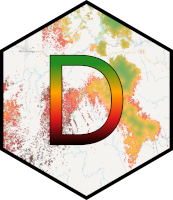
\includegraphics[width=1.5cm]{figs/logo-deforisk.png}
\end{column}
\end{columns}
\end{frame}

% %%%%%%%%%%%%%%%%%%%%%%%%%%%%%%%%%%%%%%%%%%%%%%%%%%%%%%%%%%

{
  % Use background image
  \usebackgroundtemplate{%
    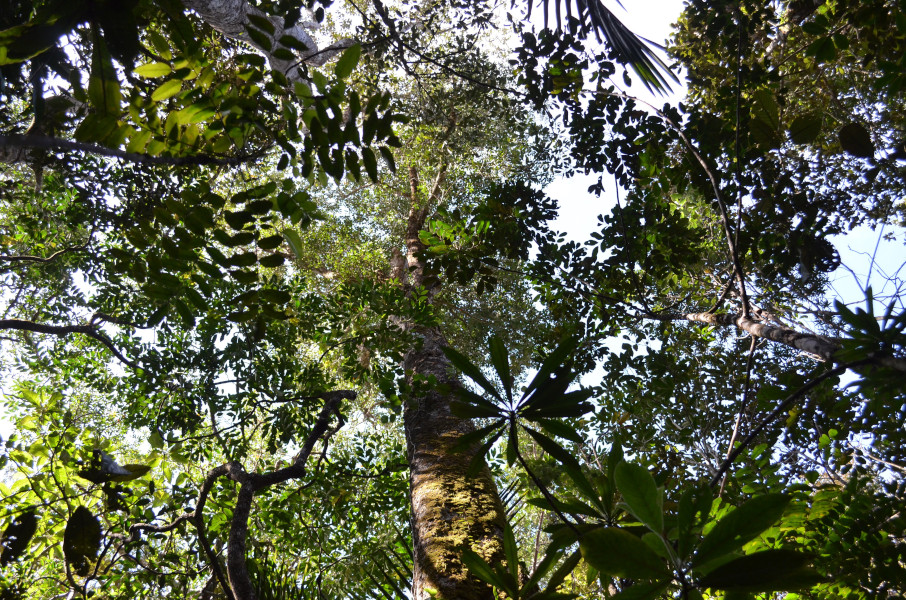
\includegraphics[keepaspectratio=true, height=\paperheight]{figs/Canopy-NC}
  }
  \setbeamertemplate{navigation symbols}{}
  % Remove shadow from block
  \setbeamertemplate{blocks}[rounded][shadow=false]
  \begin{frame}[plain]
  	\vspace*{\stretch{100}} 
    \begin{block}{}
      \begin{center}
        \ldots~Thank you for attention~\ldots \\
        \url{https://deforisk-qgis-plugin.org} \\
        \textbf{> Articles > References > Presentations} \\
        
\includegraphics[width=0.8\textwidth]{figs/partners_logos}
      \end{center}
    \end{block}
  \end{frame}
}
\end{document}
